\section{Esperimenti}
    Questo capitolo approfondisce la parte del progetto relativa ai modelli e agli esperimenti effettuati. In particolare vengono motivate le decisioni effettuate nella scelta e addestramento dei modelli, descritto il \textit{workflow} seguito per ogni modello e analizzati i risultati ottenuti.
    
    \subsection{Scelta dei modelli}
        Per identificare i modelli più adatti, è stato scelto un approccio che prevede il confronto tra sei diversi modelli di \textit{machine learning}, per confrontare le loro prestazioni e identificare i migliori. In particolare, abbiamo utilizzato per i nostri esperimenti una rete neurale, un albero di decisione, \textit{naive bayes} e tre diversi modelli di \textit{SVM} (con \textit{kernel} rispettivamente lineare, polinomiale, radiale). Abbiamo escluso solamente l'algoritmo \textit{k-means}, in quanto il nostro desiderio era effettuare solamente approcci supervisionati, avendo anche a disposizione le \textit{label} per le istanze. È stato possibile scegliere questo tipo di approccio poiché il dataset utilizzato presenta un numero esiguo di istanze e \textit{feature}, e il rispettivo \textit{train} dei vari modelli non è molto pesante in termini di tempo e risorse utilizzate. Se invece avessimo avuto un numero notevolmente maggiore di istanze e covariate, sarebbe stato più complicato sotto certi aspetti effettuare queste operazioni per tutti quanti i modelli.
        
    \subsection{Attività svolte per ogni modello}
        Per ogni modello introdotto in precedenza, si è seguito il seguente \textit{workflow}:
        \begin{enumerate}
            \item Addestramento attraverso il \textit{trainset} 
            \item Predizione sui dati contenuti nel \textit{testset}
            \item Calcolo delle metriche per il modello
            \item Calcolo della curva ROC multiclasse
        \end{enumerate}
        
        \paragraph{Train del modello e predizione} 
        Per la suddivisione dei dati in \textit{trainset} e \textit{testset} è stato deciso di selezionare il 30\% delle istanze complessive (480 istanze) in modo da rispettare la distribuzione delle istanze in base al loro valore di \textit{quality}. 
        
        L'addestramento del modello è stato effettuato svolgendo la \textit{3-repeated 10-fold cross validation}, attraverso il parametro \textit{trainControl} della funzione \textit{caret::train}. Questa opzione ci ha permesso di fare il \textit{tuning} ottimale dei parametri dei vari modelli, in quanto effettua diverse iterazioni con valori differenti al fine di trovare la misura che permette di ottimizzare la misura specificata. Per effettuare questa ottimizzazione, è stata scelta la misura di \textit{AUC}.
        
        Le predizioni invece sono state effettuate utilizzando il modello generato dal \textit{training} e il \textit{testset} precedentemente suddiviso.
    
        \paragraph{Calcolo delle metriche} Per ogni predizione effettuata, è stata poi calcolata la matrice di confusione. Il calcolo della matrice ci ha quindi permesso di determinare le differenti metriche per ogni modello generato. In particolare è stato possibile calcolare la \textit{accuracy} su tutta la matrice di confusione e \textit{precision, recall e f-measure} per ogni classe del problema. I risultati di questa fase verranno discussi nella sezione successiva.

        \paragraph{Calcolo della curva ROC} \'E stato effettuato infine il calcolo della curva \textit{ROC} e del relativo valore di \textit{AUC}. In quanto problema multiclasse, sono state generate 5 diverse curve per ogni modello: 3 relative alle classi del problema (\textit{LOW, MEDIUM, HIGH}) e le altre 2 invece alla \textit{micro average} e \textit{macro average} dei valori ottenuti.
        
        \subsubsection{Repeated 10-fold cross validation}
        Per effettuare il \textit{train} dei modelli, sono state valutate diverse tipologie differenti di metodi di \textit{resampling}. In particolare, sono state testate le prestazioni per \textit{10-fold cross validation} (d'ora in poi \textit{10-fold CV}) e \textit{k-repeated 10-fold cross validation} (considerate 10, 5 e 3 ripetizioni).
        
        Dopo aver testato i nostri modelli utilizzando la \textit{10-fold CV}, è stato deciso di sperimentare anche la \textit{10-fold CV k-repeated}. Partendo da un valore di ripetizioni k=10, abbiamo successivamente diminuito il numero di ripetizioni a k=5 e k=3. Durante lo svolgimento di queste tre prove, non sono stati riscontrati miglioramenti significativi utilizzando diversi valori di k, soprattutto non tali da giustificare l'aumento di complessità computazionale temporale.\\
        
        \begin{table}[h]
            \begin{tabular}{| c | c | c | c | c |}
                \hline
                 \textbf{Modello} & \textbf{10-fold CV} & \textbf{3 repeated} & \textbf{5 repeated} & \textbf{10 repeated}\\ 
                 \hline
                 Albero decisionale & 1.41 & 3.09 & 4.91 & 8.67 \\
                 Naive Bayes & 1.36 & 3.05 & 4.44 & 8.08 \\
                 Svm lineare & 2.96 & 3.33 & 5.03 & 9.23 \\
                 Svm polinomiale & 27.77 & 81.91 & 138.83 & 272.82 \\
                 Svm radiale & 4.86 & 13.08 & 20.97 & 41.13 \\
                 Rete neurale & 8.23 & 24.00 & 38.24 & 74.36 \\
                 \hline
            \end{tabular} 
            \caption{Tempi di calcolo con diversi metodi di resampling}
        \end{table}
        
        %Analizzando i valori ottenuti è stato osservato che con k=3 ripetizioni, venivano introdotti miglioramenti alle metriche di \textit{accuracy}, \textit{precision}, \textit{recall} e \textit{F1} durante il riconoscimento della classe \textit{HIGH}. Per questo motivo è stata utilizzata una \textit{10-fold CV 3-repeated}, considerato anche che non si è verificato un significativo aumento della complessità computazionale temporale. 
        
        I grafici successivi (figure \ref{fig:out_confrontoavg} e \ref{fig:out_confrontohigh}) mettono a confronto i valori delle metriche ottenuti attraverso la \textit{10-fold CV} (viola) con quelli risultanti dalla \textit{10-cross CV 3-repeated} (verde), per ogni metrica e modello. Sono presentati in particolare due grafici, uno relativo alla classe \textit{high} e l'altro al valore di \textit{macro average} tra tutte e tre le classi; i grafici delle altre due classi (\textit{medium, low}) non sono stati considerati per questo confronto in quanto poco significativi.
        
        \begin{figure}[!h]
            \noindent\makebox[\textwidth]{%
            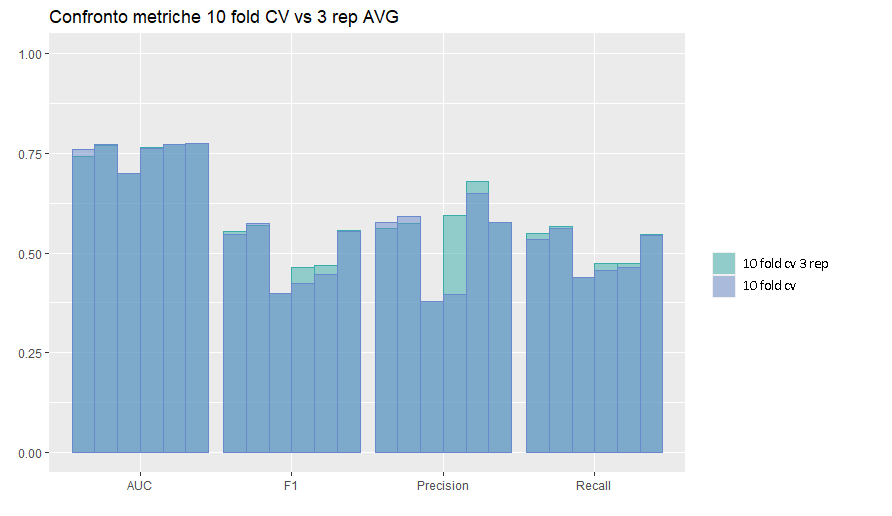
\includegraphics[width=\textwidth]{img/confronto_AVG.png}}
            \centering
            \caption{Confronto relativo alla media}
            \label{fig:out_confrontoavg}
        \end{figure}
    
        \begin{figure}[!h]
            \noindent\makebox[\textwidth]{%
            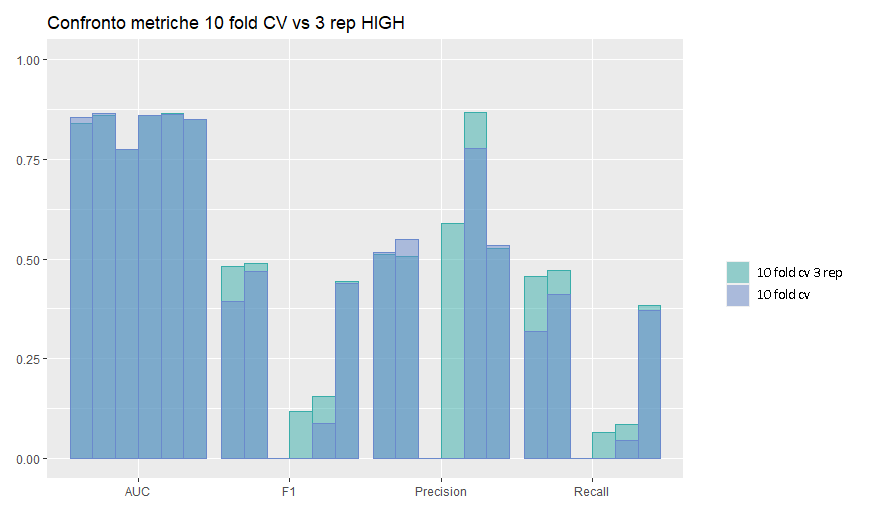
\includegraphics[width=\textwidth]{img/confronto_HIGH.png}}
            \centering
            \caption{Confronto relativo alla classe high}
            \label{fig:out_confrontohigh}
        \end{figure}
        
        \newpage
        Dai valori di \textit{macro average} (\ref{fig:out_confrontoavg}) emerge che ci sono stati piccoli cambiamenti in positivo per diversi modelli per le metriche \textit{F1}, \textit{recall} e soprattutto \textit{precision}. I cambiamenti più interessanti possono essere però osservati nel grafico successivo (\ref{fig:out_confrontohigh}), dove emerge un significativo miglioramento per tutte le metriche considerate. Uno dei modelli considerati inoltre non era in grado di classificare correttamente alcuna istanza per la classe \textit{high}, situazione che invece è cambiata con l'utilizzo della \textit{10-fold CV 3-repeated}. Questi motivi hanno quindi spinto all'adozione della \textit{10-fold CV 3-repeated} a favore della \textit{10-fold CV} senza ripetizioni.
        
        %Come miglioramento ulteriore abbiamo testato la validità di una \texit{10fold cv k repeated} invece di una \textit{10fold cv}. Siamo partiti da una \texit{10 fold cv 10 repeated} e dimezzato fino ad una \texit{10fold cv 3 repeated}, abbiamo riscontrato che in termini di miglioramento non ci sono significative differenze per il nostro modello fra 3 5 e 10 repeated, sopratutto non  così significative da giustificare l'aumento di complessità computazionale temporale. 
        %Quindi abbiamo deciso di implementare una \texit{10 fold 3 repeatet} che introduce miglioramenti in accuracy, precision, recall e F1 per la maggior parte dei modelli.
        
        \subsubsection{Downsampling}
            Essendo il numero di istanze delle varie classi sbilanciato, è stato osservato che il comportamento dei modelli risultava migliore sulla classe di maggioranza (\textit{LOW}) rispetto alle altre classi con meno istanze (\textit{MEDIUM, HIGH}). Per cercare di migliorare le prestazioni per le classi meno numerose, è stato effettuato l'addestramento delle stesse applicando una strategia di \textit{downsampling}. \'E stato scelto di utilizzare questa tecnica a favore di altre per due motivi principali: 
            \begin{itemize}
                \item Le altre tecniche creavano un numero molto alto di istanze per le classi di minoranza e andavano ad inserire numerosi istanze che non riflettevano la realtà.
                \item Essendo i valori di tutte le \textit{feature} molto vicini tra le varie classi, la creazione di altre istanze avrebbe rischiato di confondere ulteriormente il modello.
            \end{itemize}
            Analizzando i risultati ottenuti , abbiamo verificato che questa strategia ci ha permesso di migliorare le prestazioni in termini di riconoscimento della classe di minoranza \textit{HIGH}, ma ha anche peggiorato notevolmente le prestazioni per la classe \textit{MEDIUM} e anche i valori di \textit{macro average} sono risultati leggermente inferiori. Per questi motivi, è stato deciso quindi di non adottare nessuna strategia di questo tipo.

    \subsection{Analisi dei risultati ottenuti}
    La prima metrica che è stata considerata per effettuare l'analisi è la \textit{accuracy}, i quali valori sono riportati nel grafico \ref{fig:out_accuracyplot} insieme all'intervallo di confidenza. Come si può osservare dalla figura, tutti i modelli riportano sia valori che intervalli quasi sovrapposti. Considerando però che stiamo analizzando un problema multiclasse questi valori da soli non sono sufficienti per valutare la bontà del modello, in quanto non tengono conto delle diverse classi presenti. Per effettuare quindi analisi più accurate, dobbiamo considerare anche ulteriori metriche.
    
    \begin{figure}[h]
        \noindent\makebox[\textwidth]{%
        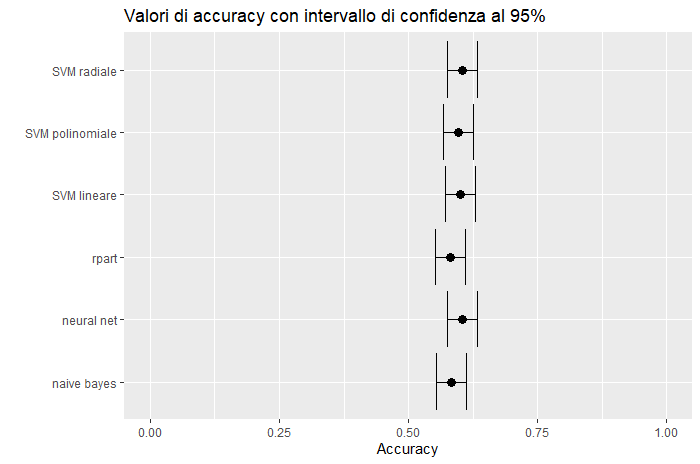
\includegraphics[scale=0.70]{img/plot_accuracy.png}}
        \centering
        \caption{Accuracy dei diversi modelli}
        \label{fig:out_accuracyplot}
    \end{figure}
    
    Avendo scelto un problema multiclasse, abbiamo ottenuto diversi valori per le metriche calcolate. Per la visualizzazione dei valori di \textit{AUC} e metriche, sono stati utilizzati grafici a barre. Sono stati generati in tutto 4 grafici di questa tipologia, 3 relativi alle classi del problema mentre il quarto prende in considerazione la \textit{macro average}, ed oguno di essi mette in relazione per ogni misura i risultati ottenuti dai vari classificatori (figura \ref{fig:out_metrics}). 
    Abbiamo valutato questa visualizzazione come la migliore poiché ci ha permesso di avere un numero minore di grafici rispetto ad altri approcci e contestualmente poter confrontare semplicemente le prestazioni per singola classe, che è stata reputata come l'informazione migliore per effettuare la valutazione.
    
    Per aggregare le metriche abbiamo optato per l'utilizzo della \textit{macro average} a dispetto della \textit{micro average}, poiché non desideravamo dare più importanza a nessuna classe nonostante lo sbilanciamento delle istanze. Avendo valutato poi singolarmente le prestazione per ogni classe e non solo il valore aggregato, è stato comunque tenuto conto del loro sbilanciamento.
    
    Osservando le metriche di \textit{marco average} si può osservare come le prestazioni medie per tutti i classificatori siano molto simili. I modelli che presentano valori aggregati peggiori sono gli alberi di decisione e, in maniera minore, \textit{SVM} lineare. 
    Al fine di analizzare nel dettaglio le cause che portano a questa differenza con gli altri modelli, è necessario guardare i valori ottenuti per ogni singola classe. In generale, si può affermare che si siano ottenute prestazioni buone sulla classe \textit{LOW} (le metriche oscillano tra il 70\% e 75\%), mentre per le altre due classi i valori sono molto meno buoni, con le metriche che oscillano intorno al 50\% per entrambe le classi. Si può osservare inoltre come per la classe di minoranza (\textit{HIGH}) alcuni classificatori non siano stati in grado di rilevare alcuna istanza. In particolare, per quanto riguarda l'albero di decisione sono stati ottenuti valori nulli.
    Questa variazione di valori può essere causata dallo sbilanciamento delle istanze in relazione alle tre classi. Come presentato in precedenza però, anche tecniche come \textit{downsampling} non sono riuscite migliorato la situazione. Si può quindi pensare che queste difficoltà siano anche dovute al fatto che i dati non siano facilmente separabili.
    
    \newpage
    
    \begin{figure}[!h]
        \noindent\makebox[\textwidth]{%
        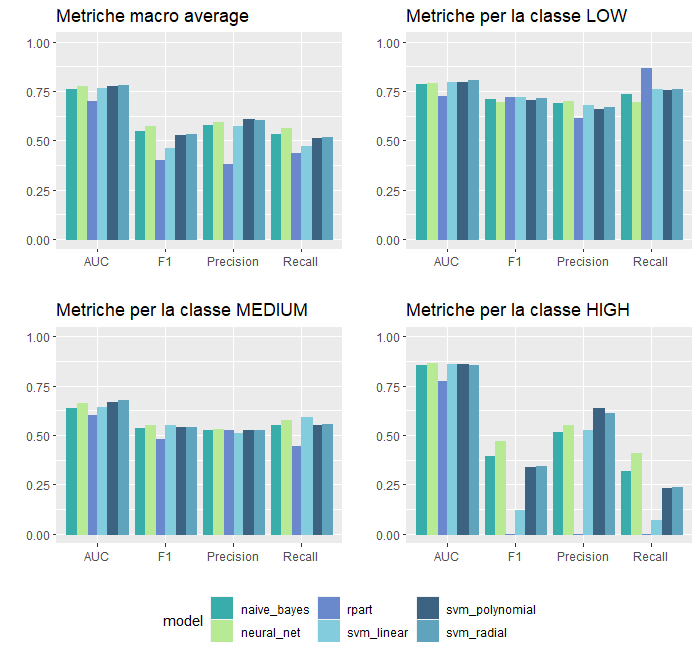
\includegraphics[scale=0.78]{img/final_metrics/finalmetrics.png}}
        \centering
        \label{fig:out_metrics}
        \caption{Metriche calcolate raggruppate per classe}
    \end{figure}

    Per ogni modello è stato anche generato il grafico relativo alle curve ROC, che rappresenta le 3 curve per le rispettive classi del problema e ulteriori 2 curve relative alle curve calcolate attraverso i valori aggregati di \textit{micro e macro average}.
    Analizzando i grafici e i valori di \textit{Area Under Curve} presentati nei grafici precedenti (\ref{fig:out_metrics}), si può osservare come le curve siano in generale molto simili tra loro e non ci sia grande discrepanza tra i differenti valori di \textit{AUC}. La curva di \textit{rpart} però risulta leggermente peggiore rispetto alle altre, e si può inoltre osservare che gli alberi presentino i valori di \textit{AUC} più bassi tra tutti i modelli.
    
    Per ogni modello inoltre emerge una differenza fra la curva relativa alla classe \textit{MEDIUM} e le altre 4. Questo valore indica la difficoltà dei modelli durante la classificazione di questo tipo di istanze, e anche in precedenza analizzando le metriche calcolate era già stato sottolineato questo aspetto. La classe \title{MEDIUM} ha performance peggiori rispetto alla classe \title{HIGH} poiché in percentuale tende a sbagliare di più in riferimento al numero di istanze totali.
    
    \newgeometry{left=0cm,right=1cm, top = 0.8cm}
    \thisfloatpagestyle{empty}
    
    \begin{table}[]
    \begin{tabular}{cc}
    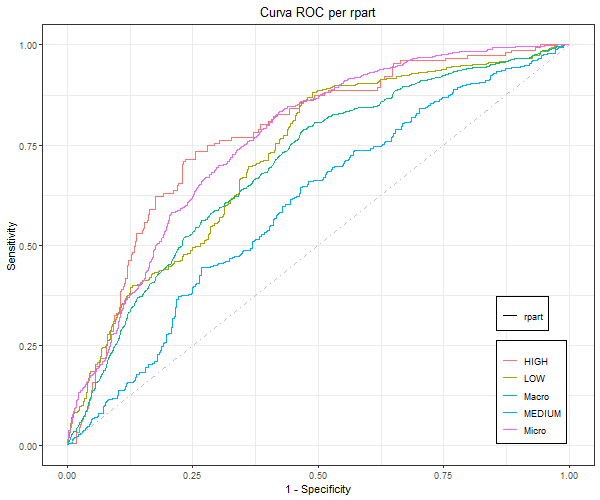
\includegraphics[width=.5\textwidth]{img/roc/roc_rpart.png} &
    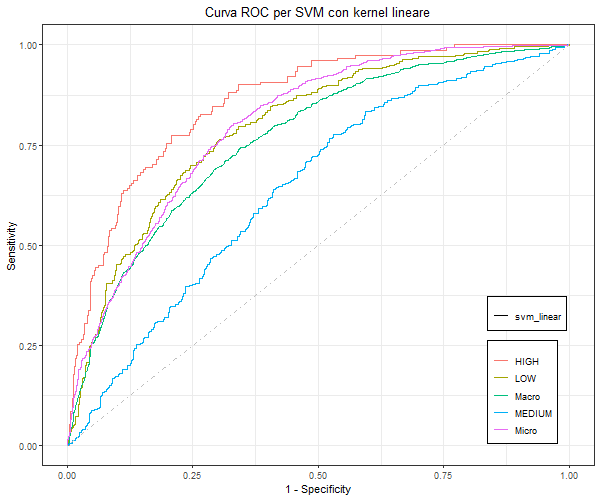
\includegraphics[width=.5\textwidth]{img/roc/roc_svml.png} \\
    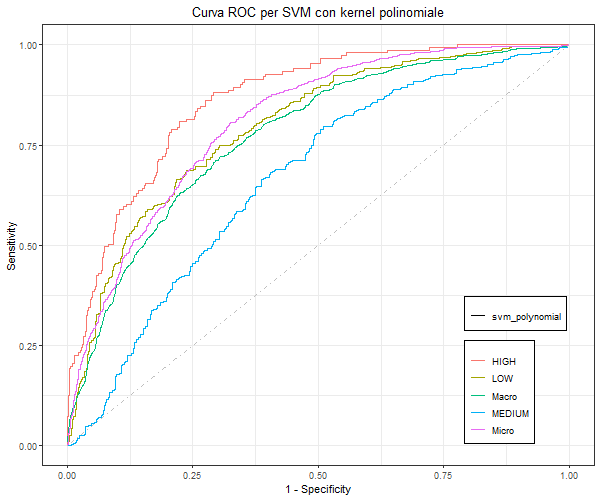
\includegraphics[width=.5\textwidth]{img/roc/roc_svmp.png} &
    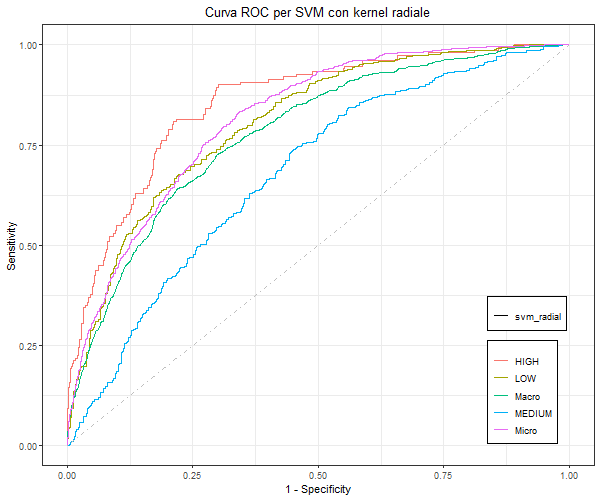
\includegraphics[width=.5\textwidth]{img/roc/roc_smvr.png} \\
    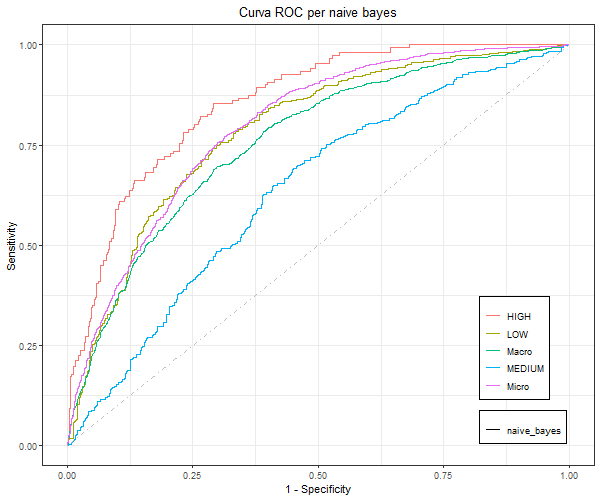
\includegraphics[width=.5\textwidth]{img/roc/roc_nb.png} &
    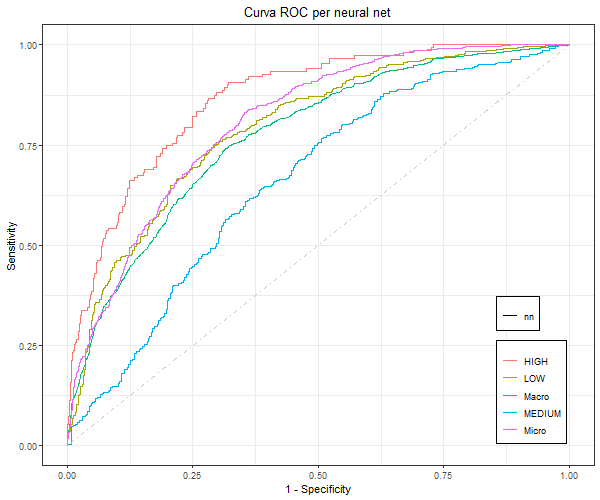
\includegraphics[width=.5\textwidth]{img/roc/roc_nn.png} \\
    \end{tabular}
    \caption{Curve ROC per tutti i modelli e per tutte le classi}
    \end{table}
    
    \restoregeometry
    \newpage
    
    Un ulteriore analisi delle prestazioni dei modelli si può effettuare considerando i loro tempi di \textit{training} e \textit{prediction}, illustrati nella tabella successiva (\ref{tab:timing}).
    Come si può osservare dai dati riportati albero decisionale, \textit{naive bayes} e SVM lineare sono i modelli più rapidi (circa 3sec), mentre il più lento in assoluto è SVM polinomiale (27x volte più lento di questi tre). SVM radiale e rete neurale invece presentano tempi più alti rispetto ai più veloci rispettivamente di 4x volte e 8x volte.
    
    Si può notare come ovviamente i modelli più semplici abbiano prestazioni ottime mentre quelli più complessi abbiamo bisogno di maggiore tempo per l'addestramento e la predizione. Si deve comunque considerare che per quanto ci sia una grande discrepanza tra i modelli, avendo utilizzato un dataset con un numero ridotto di istanze e covariate i tempi sono comunque bassi (massimo un minuto e mezzo).
    
    \begin{table}[h]
        \centering
        \begin{tabular}{| c | c |}
            \hline
             \textbf{Modello} & \textbf{Timing} \\
             \hline
             Albero decisionale & 3.09 \\
             Naive Bayes & 3.05 \\
             Svm lineare & 3.33 \\
             Svm polinomiale & 81.91 \\
             Svm radiale & 13.08 \\
             Rete neurale & 24.00 \\
             \hline
        \end{tabular} 
        \caption{Tempi di calcolo con diversi metodi di resampling}
        \label{tab:timing}
    \end{table}
    
    Considerando tutti gli aspetti presentati è quindi possibile quindi delineare quale siano i modelli che possano essere considerati come i migliori. Oltre alle prestazioni raggiunte, è importante considerare anche il costo per ottenerle, al fine di avere il giusto \textit{trade off} tra tempi e correttezza delle predizioni del modello.
    
    L'albero decisionale è in assoluto il modello più semplice e veloce tra quelli presentati, ma questo si traduce anche in prestazioni non ottimali. Come già presentato in precedenza infatti, non è stato in grado di classificare alcuna istanza di tipo \textit{HIGH}, oltre a non avere prestazioni come gli altri relative a tutte le altre classi. Per questo motivo, si può affermare che, nonostante i suoi pregi, non possa essere considerato in questo caso un buon classificatore.
    
    \textit{Naive Bayes} è il modello giudicato come migliore tra quelli presentati, poiché si rilevano ottime prestazioni mantenendo però bassa complessità computazionale. Come si può osservare dai grafici infatti, le sue prestazioni sono in linea con quelle degli altri classificatori più complessi ma presenta il tempo in assoluto più basso per addestramento e predizione.
    
    Un modello che ha ottenuto prestazioni inferiori rispetto agli altri è \textit{SVM} lineare, che come gli alberi ha presentato problemi di classificazione per la classe \textit{HIGH}, ma nonostante ciò è un buon \textit{trade-off} tra risultati ottenuti e complessità computazionale. Per questo può essere considerato come un discreto classificatore, nonostanze prestazioni inferiori agli altri modelli.
    
    Per quanto riguarda \textit{SVM} polinomiale invece, presenta ottime prestazioni dal punto di vista delle metriche. Il fattore che penalizza però molto questo classificatore è il tempo di addestramento e predizione, che è in assoluto quello più alto riscontrato tra tutti i modelli analizzati. Possiamo quindi considerare altri classificatori (come ad esempio \textit{naive bayes}, reti neurali e \textit{SVM} radiale) come migliori poiché, a fronte di prestazioni simili, si ha una complessità computazionale decisamente minore.
    
    \textit{SVM} radiale e reti neurali possono infine essere considerati entrambi come buoni classificatori. Per quanto riguarda il primo abbiamo ottenuto prestazioni in linea con i modelli migliori, a fronte di una complessità abbastanza bassa. La rete neurale invece, nonostante tempi di addestramento e predizione tra i più alti, è stato il modello che è stato più in grado di effettuare una discriminazione corretta delle istanze \textit{HIGH}. Per i motivi presentati, questi due classificatori possono essere considerati quindi i migliori considerati dopo \textit{naive bayes}.
    
    
    